\chapter{Regresión}

\section{Introducción}
Analizado el dataset 'California', en esta sección se desarrollarán diferentes modelos predictivos a partir del mismo. \\

Comenzando con el estudio y la elaboración de modelos lineales simples, posteriormente se generarán modelos más complejos, modelos no lineales y finalmente modelos basados en K-NN, todos con el objetivo explicar la variable dependiente (MedianHouseValue).




\section{Elaborar modelos lineales simples.}

Se presenta un dataset formado por más de 5 variables, por ello es necesario realizar un estudio que permita determinar aquellas 5 más relevantes.\\

Este estudio consistirá en la generación de los diferentes modelos lineales simples, con el fin de detectar aquellas variable independientes capaces de explicar un considerable porcentaje de la variable dependiente. \\

Cada modelo generado es evaluado:
\begin{table}[!h]
	\begin{tabular}{l|llll}
		Modelo Lineal                           & R\textasciicircum{}2 & R\textasciicircum{}2 Ajustado & RMSE   & p-value   \\ \hline
		MedianHouseValue $\sim$Longitude        & 0.002113             & 0.002065                      & 115300 & 3.923e-11 \\
		MedianHouseValue $\sim$Latitude         & 0.02078              & 0.02073                       & 114200 & 2.2e-16   \\
		MedianHouseValue $\sim$HousingMedianAge & 0.01116              & 0.01111                       & 114800 & 2.2e-16   \\
		MedianHouseValue $\sim$TotalRooms       & 0.018                & 0.01795                       & 114400 & 2.2e-16   \\
		MedianHouseValue $\sim$TotalBedrooms    & 0.00256              & 0.002511                      & 115300 & 3.52e-13  \\
		MedianHouseValue $\sim$Population       & 0.0006076            & 0.0005592                     & 115400 & 0.0003976 \\
		MedianHouseValue $\sim$Households       & 0.004335             & 0.004287                      & 115100 & 2.2e-16   \\
		MedianHouseValue $\sim$MedianIncome     & 0.4734               & 0.4734                        & 83740  & 2.2e-16  
	\end{tabular}
\end{table}

\newpage
Se representan gráficamente los diferentes modelos generados:

\begin{figure}[!tbh]
	\centering
	\begin{subfigure}{0.5\textwidth}
	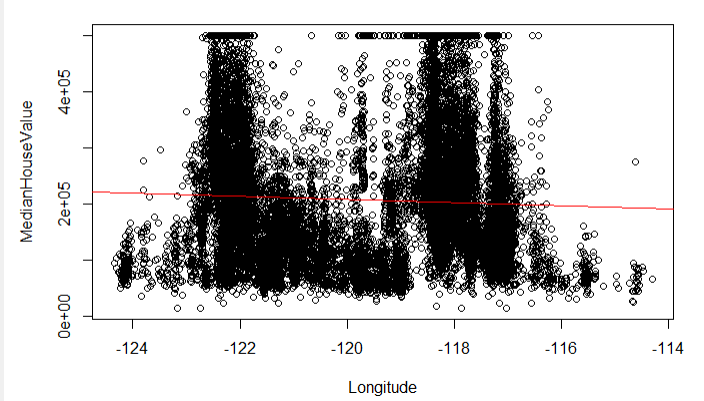
\includegraphics[width=1\linewidth]{figures/regre_1}
\caption{}
\label{fig:regre1}
	\end{subfigure}\hfil % <-- added
	\begin{subfigure}{0.5\textwidth}
	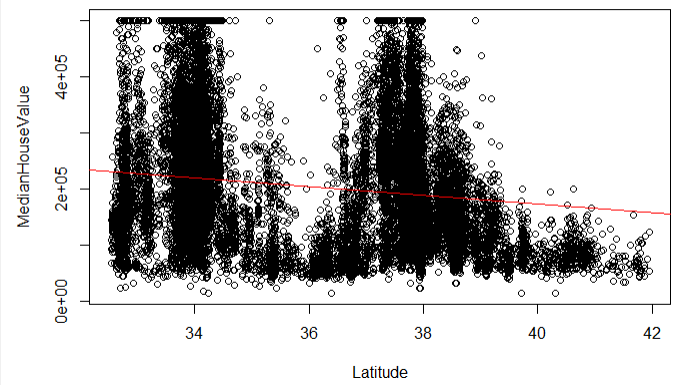
\includegraphics[width=1\linewidth]{figures/regre_2}
\caption{}
\label{fig:regre2}
	\end{subfigure}\hfil % <-- added
	
	\medskip
	
	\begin{subfigure}{0.5\textwidth}
	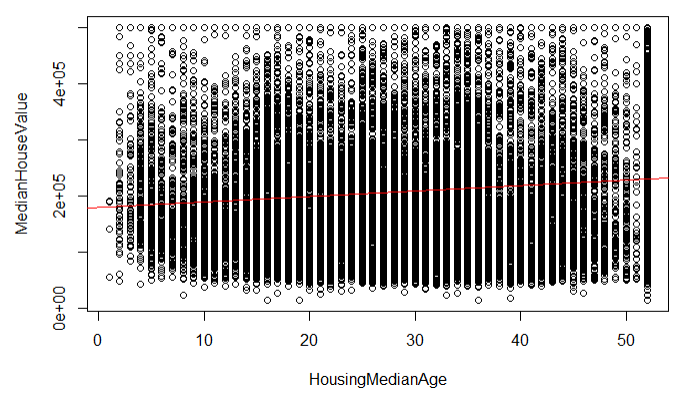
\includegraphics[width=1\linewidth]{figures/regre_3}
\caption{}
\label{fig:regre3}
	\end{subfigure}\hfil % <-- added
	\begin{subfigure}{0.5\textwidth}
	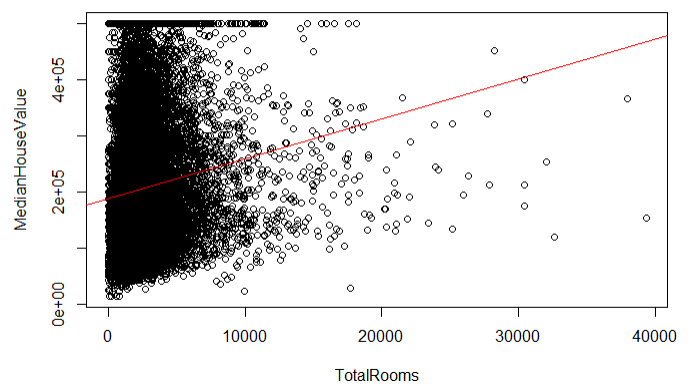
\includegraphics[width=1\linewidth]{figures/regre_4}
\caption{}
\label{fig:regre4}
	\end{subfigure}\hfil % <-- added
	
	\medskip
	
	\begin{subfigure}{0.5\textwidth}
	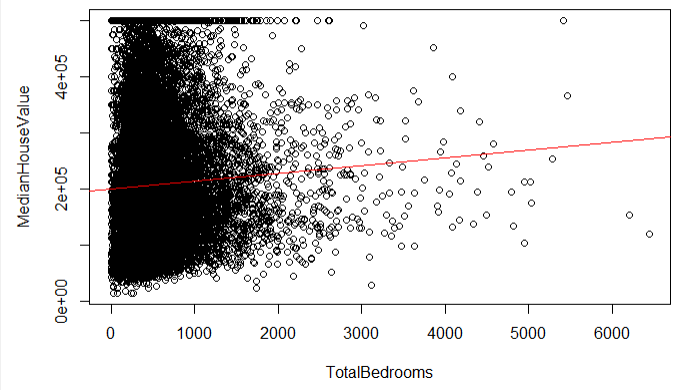
\includegraphics[width=1\linewidth]{figures/regre_5}
\caption{}
\label{fig:regre5}
	\end{subfigure}\hfil % <-- added
	\begin{subfigure}{0.5\textwidth}
	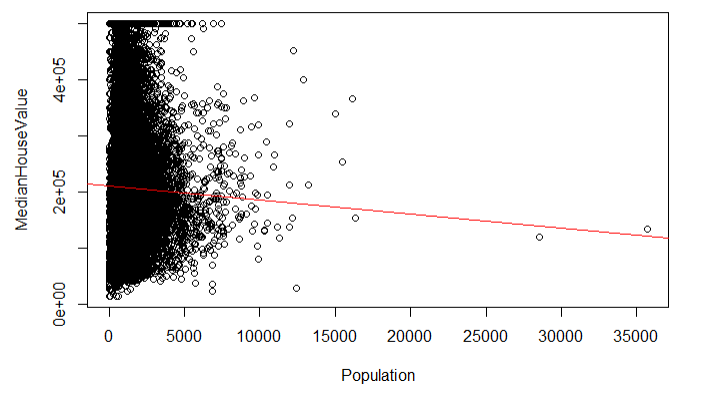
\includegraphics[width=1\linewidth]{figures/regre_6}
\caption{}
\label{fig:regre6}
	\end{subfigure}\hfil % <-- added

	\medskip

\begin{subfigure}{0.5\textwidth}
	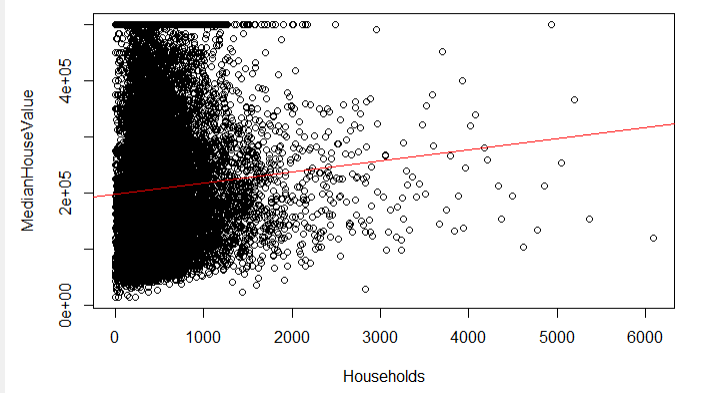
\includegraphics[width=1\linewidth]{figures/regre_7}
	\caption{}
	\label{fig:regre7}
\end{subfigure}\hfil % <-- added
\begin{subfigure}{0.5\textwidth}
	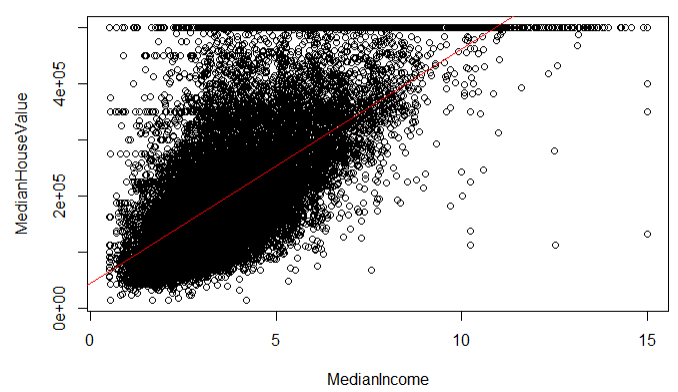
\includegraphics[width=1\linewidth]{figures/regre_8}
	\caption{}
	\label{fig:regre8}
\end{subfigure}\hfil % <-- added
	
	\caption{Modelos lineales simples}
	\label{lm}
\end{figure}





\newpage
Se observa que todos los modelos lineales generados, exceptuando el que trabaja con la variable independiente 'MedianIncome', presentan un valor de R cuadrado ajustado muy cercano a 0, lo que permite asumir que estas variable por si mismas no pueden llegar a explicar la variable dependiente 'MedianHouseValue'.\\

Fijando la atención en el caso del modelo con la variable 'MedianIncome', se presenta un valor R cuadrado ajustado próximo al 0.5, lo que se traduce en que esta variable por si sola es capaz de explicar gran parte de la variable dependiente, pero no lo suficiente. La importancia de esta variable será de utilidad para la elaboración de modelos más complejos.\\

Evaluando las métricas resultantes se observa que las 5 variables que mejor explican la variable dependiente son:
\begin{table}[!h]
	\begin{tabular}{l|llll}
		Modelo Lineal                           & R\textasciicircum{}2 & R\textasciicircum{}2 Ajustado & RMSE   & p-value \\ \hline
		MedianHouseValue $\sim$MedianIncome     & 0.4734               & 0.4734                        & 83740  & 2.2e-16 \\
		MedianHouseValue $\sim$Latitude         & 0.02078              & 0.02073                       & 114200 & 2.2e-16 \\
		MedianHouseValue $\sim$TotalRooms       & 0.018                & 0.01795                       & 114400 & 2.2e-16 \\
		MedianHouseValue $\sim$HousingMedianAge & 0.01116              & 0.01111                       & 114800 & 2.2e-16 \\
		MedianHouseValue $\sim$Households       & 0.004335             & 0.004287                      & 115100 & 2.2e-16
	\end{tabular}
\end{table}


Para finalizar este apartado se determinará cual es el mejor de estos modelos comprobando cual de ellos obtiene el menor error cuadrático medio (RMSE) en los 5 folds propuestos para este dataset.
\begin{table}[!h]
	\begin{tabular}{l|llll}
		Modelo Lineal                           & R\textasciicircum{}2 & R\textasciicircum{}2 Ajustado & RMSE   & 5-fold RMSE \\ \hline
		MedianHouseValue $\sim$MedianIncome     & 0.4734               & 0.4734                        & 83740  & 7006888908  \\
		MedianHouseValue $\sim$Latitude         & 0.02078              & 0.02073                       & 114200 & 13037618917 \\
		MedianHouseValue $\sim$TotalRooms       & 0.018                & 0.01795                       & 114400 & 13074242952 \\
		MedianHouseValue $\sim$HousingMedianAge & 0.01116              & 0.01111                       & 114800 & 13164908193 \\
		MedianHouseValue $\sim$Households       & 0.004335             & 0.004287                      & 115100 & 13256188343
	\end{tabular}
\end{table}

\vspace{0.5cm}
El modelo lineal creado en función de 'MedianIncome' ha obtenido el menor error cuadrático medio en la validación cruzada de 5-folds, confirmando de nuevo que es el mejor modelo de regresión lineal simple posible.




\newpage
\section{Elaborar modelos regresión lineal múltiple}
En este apartado se analizarán y crearán diferentes modelos que consideren varias variables independientes para explicar la variable dependiente. Para ello se procederá mediante un método descendiente, el cual consiste en partir de un modelo lineal que considere todas las posibles variables independientes y, a partir de este, se buscará la obtención de modelos progresivamente mejores mediante la eliminación de variables y/o añadiendo términos no lineales.\\

El resultado de este primer modelo es el siguiente:
\begin{figure}[!h]
	\centering
	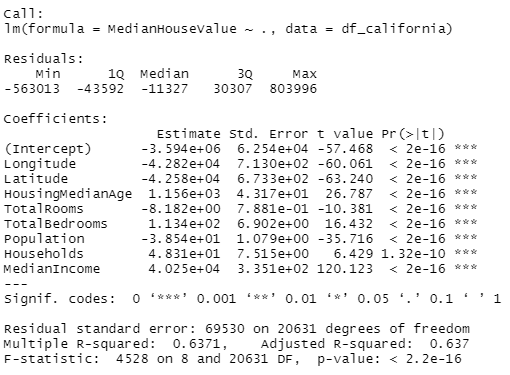
\includegraphics[width=0.7\linewidth]{figures/fit_multi1}
	\caption{}
	\label{fig:fitmulti1}
\end{figure}

Media RMSE del modelo lineal múltiple sobre 5-fold: 4844365688
\vspace{0.5cm}
\begin{table}[!h]
	\centering
	\begin{tabular}{llll}
		R\textasciicircum{}2 & R\textasciicircum{}2 Ajustado & RMSE  & 5-fold RMSE \\ \hline
		0.6371               & 0.637                         & 69530 & 4844365688 
	\end{tabular}
\end{table}

Se observa que el modelo generado ofrece mejor rendimiento frente a cualquiera de los modelos lineales simples generados en el apartado anterior. Por otro lado, los valores p-value del test de Wall no presentan valores significativos en ninguno de los casos, lo que complica la identificación de una variable de la que se pudiera prescindir.\\

Debido a esta situación, el estudio de nuevos modelos a partir de este mediante la eliminación de variables se realizará comenzando por aquellas variables que no fueron seleccionadas para el estudio de los 5 modelos lineales simples anteriores. \\

Por ello se comienza eliminando la variable independiente 'Longitude', generando el siguiente modelo:
\begin{figure}[!h]
	\centering
	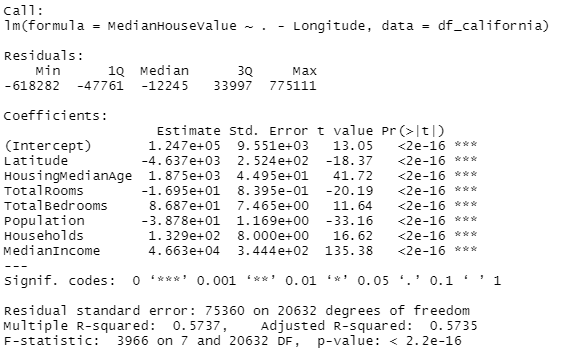
\includegraphics[width=0.7\linewidth]{figures/fit_multi_2}
	\caption{}
	\label{fig:fitmulti2}
\end{figure}

Media RMSE del modelo lineal múltiple sobre 5-fold: 5688531919
\vspace{0.5cm}
\begin{table}[!h]
	\centering
	\begin{tabular}{llll}
		R\textasciicircum{}2 & R\textasciicircum{}2 Ajustado & RMSE  & 5-fold RMSE \\ \hline
		0.5737               & 0.5735                        & 75360 & 5688531919 
	\end{tabular}
\end{table}

La eliminación de 'Longitude' da lugar a un modelo con un peor R cuadrado ajustado respecto al anterior, por ello se opta por conservar esta variable y probar eliminando la siguiente no elegida anteriormente: 'Population'.
\begin{figure}[!h]
	\centering
	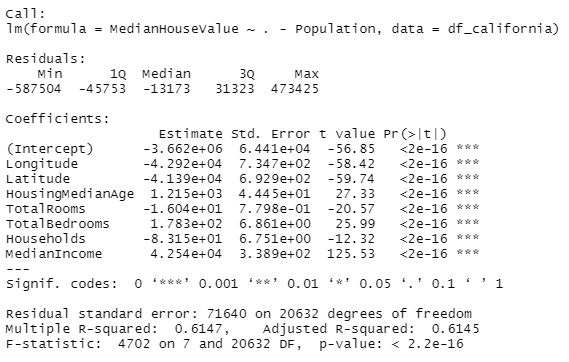
\includegraphics[width=0.7\linewidth]{figures/fit_multi_3}
	\caption{}
	\label{fig:fitmulti3}
\end{figure}

Media RMSE del modelo lineal múltiple sobre 5-fold: 5130744110
\vspace{0.5cm}
\begin{table}[!h]
	\centering
	\begin{tabular}{llll}
		R\textasciicircum{}2 & R\textasciicircum{}2 Ajustado & RMSE  & 5-fold RMSE \\ \hline
		0.6147               & 0.6145                        & 71640 & 5130744110 
	\end{tabular}
\end{table}

En este caso los resultados son levemente inferiores. Se prueba por último la eliminación de la variable 'TotalBedrooms', la última de las no elegidas entre las 5 variables más relevantes en la sección anterior.
\begin{figure}[!h]
	\centering
	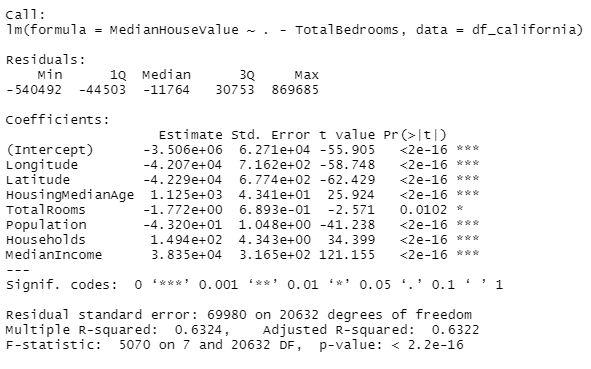
\includegraphics[width=0.7\linewidth]{figures/fit_multi_4}
	\caption{}
	\label{fig:fitmulti4}
\end{figure}

Media RMSE del modelo lineal múltiple sobre 5-fold: 4909112109
\vspace{0.5cm}
\begin{table}[!h]
	\centering
	\begin{tabular}{llll}
		R\textasciicircum{}2 & R\textasciicircum{}2 Ajustado & RMSE  & 5-fold RMSE \\ \hline
		0.6324               & 0.6322                        & 69980 & 4909112109 
	\end{tabular}
\end{table}

De nuevo los resultados son levemente peores. 
Si la eliminación de aquellas variables que no fueron seleccionada como relevantes da lugar a peores modelos podemos prácticamente deducir que con la eliminación de cada una de las 5 variables restantes los modelos obtenidos también será peores. Por ello se opta por la realización de modelos que involucren a todas las variables, pero añadiendo términos no lineales.\\

\newpage
Siendo 'MedianIncome' la variable que mejor explica la variable dependiente comencemos añadiéndola elevada al cuadrado:
\begin{figure}[!h]
	\centering
	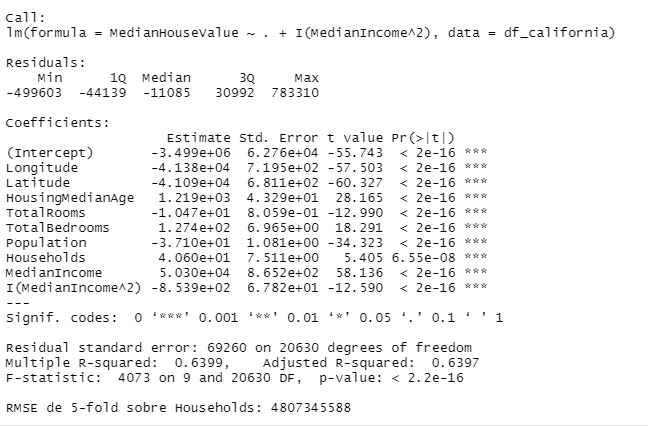
\includegraphics[width=0.7\linewidth]{figures/fit_multi_5}
	\caption{}
	\label{fig:fitmulti5}
\end{figure}

\begin{table}[!h]
	\centering
	\begin{tabular}{llll}
		R\textasciicircum{}2 & R\textasciicircum{}2 Ajustado & RMSE  & 5-fold RMSE \\ \hline
		0.6399               & 0.6397                        & 69260 & 4807345588 
	\end{tabular}
\end{table}

Se observa la generación de un modelo levemente superior respecto al formado por todas las variables.
Se prueba a continuación elevándola a 4:
\begin{figure}[!h]
	\centering
	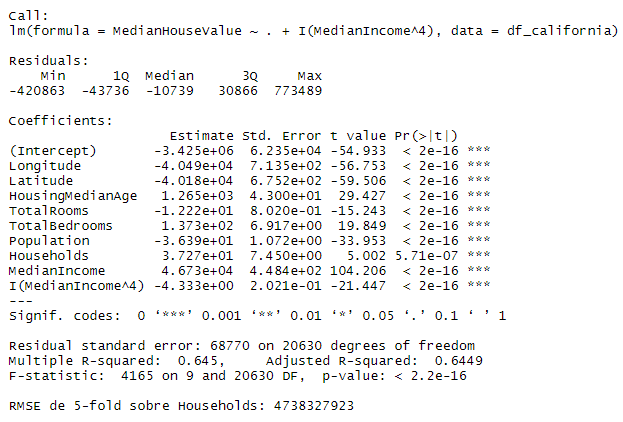
\includegraphics[width=0.7\linewidth]{figures/fit_multi_6}
	\caption{}
	\label{fig:fitmulti6}
\end{figure}

\begin{table}[!h]
	\centering
	\begin{tabular}{llll}
		R\textasciicircum{}2 & R\textasciicircum{}2 Ajustado & RMSE  & 5-fold RMSE \\ \hline
		0.645                & 0.6449                        & 68770 & 4738327923 
	\end{tabular}
\end{table}

Se produce una muy leve mejora, seguir por este camino no dará lugar a mejores resultados. 
Dado que tener en cuenta una de la variable más representativa origina modelos con mejores resultamos, añadamos el producto de las dos siguientes variables determinada como más relevante, 'Latitude' y 'TotalRooms':
\begin{figure}[!h]
	\centering
	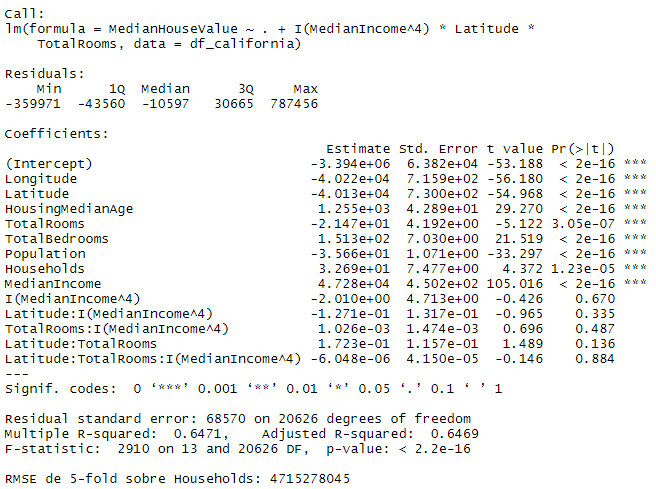
\includegraphics[width=0.7\linewidth]{figures/fit_multi_7}
	\caption{}
	\label{fig:fitmulti7}
\end{figure}

\begin{table}[!h]
	\centering
	\begin{tabular}{llll}
		R\textasciicircum{}2 & R\textasciicircum{}2 Ajustado & RMSE  & 5-fold RMSE \\ \hline
		0.6471               & 0.6469                        & 68570 & 4715278045 
	\end{tabular}
\end{table}

Se observa un modelo con unos mejores resultados, sin embargo, al observar los valores 'p-value' se desconfía de algunas variables añadidas en la multiplicación. \\

Por ello se considera en eliminar la variable 'Latitude' multiplicando.
\newpage
\begin{figure}[!h]
	\centering
	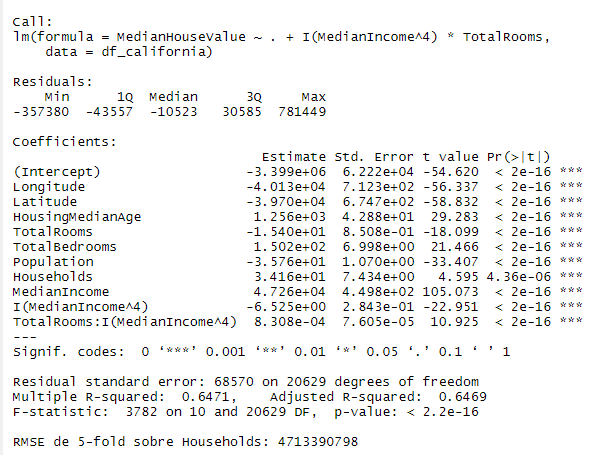
\includegraphics[width=0.7\linewidth]{figures/fit_multi_8}
	\caption{}
	\label{fig:fitmulti8}
\end{figure}

\begin{table}[!h]
	\centering
	\begin{tabular}{llll}
		R\textasciicircum{}2 & R\textasciicircum{}2 Ajustado & RMSE  & 5-fold RMSE \\ \hline
		0.6471               & 0.6469                        & 68570 & 4713390798 
	\end{tabular}
\end{table}

Efectivamente la variable 'Latitude' multiplicando no aportaba ninguna mejor.\\

Se decide continuar agregando los siguientes términos más significativos multiplicando, 'HousingMedianAge' y 'Households'
\begin{figure}[!h]
	\centering
	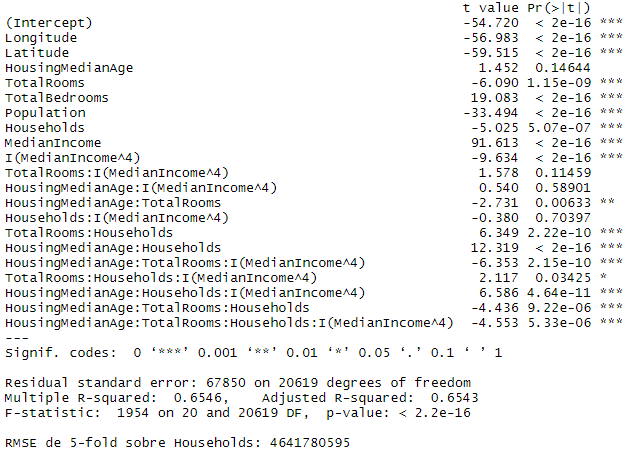
\includegraphics[width=0.7\linewidth]{figures/fit_multi_9}
	\caption{}
	\label{fig:fitmulti9}
\end{figure}

\begin{table}[!h]
	\centering
	\begin{tabular}{llll}
		R\textasciicircum{}2 & R\textasciicircum{}2 Ajustado & RMSE  & 5-fold RMSE \\ \hline
		0.6546               & 0.6543                        & 67850 & 4641780595 
	\end{tabular}
\end{table}

De nuevo se mejoran los resultados, pero se observa que en varios casos en los que interviene I($MedianIncome ^{4} $) aparecen valores de 'p-value' que añaden desconfianza a este término, por ello se decide probar sin elevarlo a 4.
\begin{figure}[!h]
	\centering
	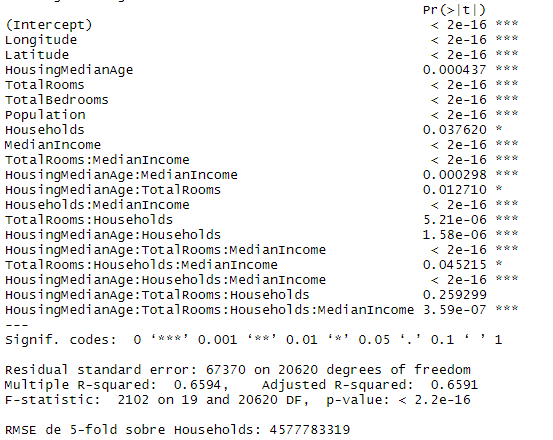
\includegraphics[width=0.7\linewidth]{figures/fit_multi_10}
	\caption{}
	\label{fig:fitmulti10}
\end{figure}

\begin{table}[!h]
	\centering
	\begin{tabular}{llll}
		R\textasciicircum{}2 & R\textasciicircum{}2 Ajustado & RMSE  & 5-fold RMSE \\ \hline
		0.6594               & 0.6591                        & 67370 & 4577783319 
	\end{tabular}
\end{table}

La suposición era correcta y de nuevo han mejorado los resultados. Sin embargo, los valores *p-value* indican que no es necesaria la presencia de algunos de los términos del modelo (caso de la multiplicación de HousingMedianAge:TotalRooms:Households).\\ 

Finalmente nos quedamos con este último modelo como mejor modelo múltiple generado.








\newpage
\section{Aplicar el algoritmo k-NN para regresión}
En esta sección se elaboran y estudian modelos basados en k-NN. Este estudio se realizará sobre el mejor modelo obtenido en la sección anterior con diferentes valores de k (número de vecinos más cercanos), con el objetivo de determinar el valor de k más cercano al óptimo. \\

Por tanto la siguiente tabla recoge, para diferentes valores de k, el valor de RMSE obtenido tras realizar la validación cruzada de 5-folds, para cada caso, junto con la media de estos resultados. Utilizando en todos ellos el mejor modelo múltiple conseguido en el apartado anterior: MedianHouseValue ~ . +MedianIncome*TotalRooms*HousingMedianAge*Households.

\begin{table}[!h]
	\begin{tabular}{l|llllll}
		k  & Fold 1     & Fold 2     & Fold 3     & Fold 4     & Fold 5     & Media RMSE          \\ \hline
		5  & 4541760347 & 4530471424 & 4565272732 & 4385513226 & 4745290191 & 4553661584          \\
		7  & 4283086269 & 4381302961 & 4329091939 & 4106711363 & 4473274188 & 4314693344          \\
		10 & 4157055323 & 4196558009 & 4173551945 & 4018343901 & 4313895845 & 4171881005          \\
		20 & 4046433324 & 4096849734 & 4069779207 & 3898401005 & 4167615566 & \textbf{4051576629} \\
		25 & 4046433324 & 4096849734 & 4069779207 & 3898401005 & 4162774625 & 4054847579          \\
		50 & 4161252917 & 4184933077 & 4160816036 & 4002315397 & 4258437778 & 4153551041         
	\end{tabular}
\end{table}


Siendo la media del error RMSE obtenida en el modelo de regresión múltiple de 4577783319 sobre 5-folds, determinamos que con un k=5 ya se obtienen mejores resultados con el uso de k-NN en la validación cruzada 5-folds, siendo el valor óptimo de k un valor cercano a 20.
\begin{figure}[!h]
	\centering
	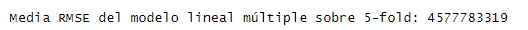
\includegraphics[width=1.2\linewidth]{figures/media}
	\caption{}
	\label{fig:media}
\end{figure}




\newpage
\section{Comparar los resultados de los dos algoritmos de regresión múltiple}
Finalmente, se comparan los resultados de los algoritmos de regresión múltiple, k-NN y, adicionalmente, el modelo M5', cuyos resultados han sido aportadas por el profesorado, ya que no ha sido tratado en el desarrollo de este proyecto.
Estas comparativas se realizan con las mismas condiciones sobre cada algoritmo, no se mantienen consideraciones específicas, se trabaja con todas las variables (MedianHouseValue ~ .).\\

En primer lugar, se utiliza el test de Wilcoxon, un test no paramétrico que permite determinar si existes relación entre dos muestras. De esta forma, se observa si existen diferencias significativas entre la regresión lineal múltiple y k-NN. La comparativa se realiza utilizando RMSE como medida de precisión para cada modelo.
Fijando el nivel de significancia en 0.05, si el p-value resultante está por debajo de este nivel, se rechaza la hipótesis nula del test, lo que indica que uno de los modelos da unos resultados significativamente distintos a los del otro modelo.

Test modelo lineal (R+) vs modelo k-NN:(R-)
\begin{table}[!h]
	\centering
	\begin{tabular}{lll}
		R+ & R- & p-value   \\ \hline
		78 & 93 & 0.7660294
	\end{tabular}
\end{table}


Puesto que el p-value resultante posee un valor superior al nivel de significancia, no es posible rechazar que ambos algoritmos ofrecen resultados similares.\\

A continuación, se utiliza el test de Friedman para determinar si existen diferencias significativas entre los 3 modelos:

Friedman rank sum test
\begin{table}[!h]
	\centering
	\begin{tabular}{lll}
		chi-squared & df & p-value \\ \hline
		8.4444      & 2  & 0.01467
	\end{tabular}
\end{table}

En este caso el valor de p-value si se sitúa por debajo del nivel de significancia, por ello se rechaza la hipótesis nula, es decir, existe al menos diferencias significativas entre un par de los algoritmos evaluados.
Finalmente aplicamos el test post-hoc de Holm para averiguar qué par es diferente y cuales se pueden considerar similares

\begin{table}[!h]
	\centering
	\begin{tabular}{l|ll}
		Modelos Regresión & Lineal Múltiple & k-NN  \\ \hline
		k-NN              & 0.580           & -     \\
		M5'               & 0.081           & 0.108
	\end{tabular}
\end{table}


Se observa la existencia de diferencias significativas entre M5' con la regresión lineal múltiple, pues su valor de p-value no superar el nivel de significancia. Los dos pares restantes poseen similitud, destacando similitud entre k-nn y regresión lineal múltiple.




